%% This is file `elsarticle-template-1-num.tex',
%%
%% Copyright 2009 Elsevier Ltd
%%
%% This file is part of the 'Elsarticle Bundle'.
%% ---------------------------------------------
%%
%% It may be distributed under the conditions of the LaTeX Project Public
%% License, either version 1.2 of this license or (at your option) any
%% later version.  The latest version of this license is in
%%    http://www.latex-project.org/lppl.txt
%% and version 1.2 or later is part of all distributions of LaTeX
%% version 1999/12/01 or later.
%%
%% The list of all files belonging to the 'Elsarticle Bundle' is
%% given in the file `manifest.txt'.
%%
%% Template article for Elsevier's document class `elsarticle'
%% with numbered style bibliographic references
%%
%% $Id: elsarticle-template-1-num.tex 149 2009-10-08 05:01:15Z rishi $
%% $URL: http://lenova.river-valley.com/svn/elsbst/trunk/elsarticle-template-1-num.tex $
%%
\documentclass[final,5p,times,twocolumn]{elsarticle}
%% Use the option review to obtain double line spacing
%% \documentclass[preprint,review,12pt]{elsarticle}

%% Use the options 1p,twocolumn; 3p; 3p,twocolumn; 5p; or 5p,twocolumn
%% for a journal layout:
%% \documentclass[final,1p,times]{elsarticle}
%% \documentclass[final,1p,times,twocolumn]{elsarticle}
%% \documentclass[final,3p,times]{elsarticle}
%% \documentclass[final,3p,times,twocolumn]{elsarticle}
%% \documentclass[final,5p,times]{elsarticle}
%% \documentclass[final,5p,times,twocolumn]{elsarticle}

%% if you use PostScript figures in your article
%% use the graphics package for simple commands
%%\usepackage{graphics}
%% or use the graphicx package for more complicated commands
%%\usepackage{graphicx}
%% or use the epsfig package if you prefer to use the old commands
%% \usepackage{epsfig}

%% The amssymb package provides various useful mathematical symbols
\usepackage{amssymb}
%% The amsthm package provides extended theorem environments
%% \usepackage{amsthm}

%% The lineno packages adds line numbers. Start line numbering with
%% \begin{linenumbers}, end it with \end{linenumbers}. Or switch it on
%% for the whole article with \linenumbers after \end{frontmatter}.
%% \usepackage{lineno}

%% natbib.sty is loaded by default. However, natbib options can be
%% provided with \biboptions{...} command. Following options are
%% valid:

%%   round  -  round parentheses are used (default)
%%   square -  square brackets are used   [option]
%%   curly  -  curly braces are used      {option}
%%   angle  -  angle brackets are used    <option>
%%   semicolon  -  multiple citations separated by semi-colon
%%   colon  - same as semicolon, an earlier confusion
%%   comma  -  separated by comma
%%   numbers-  selects numerical citations
%%   super  -  numerical citations as superscripts
%%   sort   -  sorts multiple citations according to order in ref. list
%%   sort&compress   -  like sort, but also compresses numerical citations
%%   compress - compresses without sorting
%%
%% \biboptions{comma,round}

% \biboptions{}


\journal{Information and Software Technology}

\begin{document}

\begin{frontmatter}

%% Title, authors and addresses

%% use the tnoteref command within \title for footnotes;
%% use the tnotetext command for the associated footnote;
%% use the fnref command within \author or \address for footnotes;
%% use the fntext command for the associated footnote;
%% use the corref command within \author for corresponding author footnotes;
%% use the cortext command for the associated footnote;
%% use the ead command for the email address,
%% and the form \ead[url] for the home page:
%%
%% \title{Title\tnoteref{label1}}
%% \tnotetext[label1]{}
%% \author{Name\corref{cor1}\fnref{label2}}
%% \ead{email address}
%% \ead[url]{home page}
%% \fntext[label2]{}
%% \cortext[cor1]{}
%% \address{Address\fnref{label3}}
%% \fntext[label3]{}

\title{Evaluating the Health of Open Source Components}

%% use optional labels to link authors explicitly to addresses:
%% \author[label1,label2]{<author name>}
%% \address[label1]{<address>}
%% \address[label2]{<address>}

\author[UU]{Ivan Zaytsev\corref{cor1}}
\ead{i.zaytsev@students.uu.nl}
\author[UU]{Slinger Jansen}
\ead{s.jansen@cs.uu.nl}
\cortext[cor1]{Corresponding author. Address: Department of Information and Computing Sciences, University of Utrecht, P.O. Box 80.089, 3508TB Utrecht, The Netherlands. Tel.: +31 (0)30 253 98 96.}
\address[UU]{Department of Information and Computer Sciences, Utrecht University, Utrecht, The Netherlands}


\begin{abstract}
\textit{Context}: Implementing open source components into commercial applications has many advantages for software developers. However, an unforeseen decline in health of the supplying community can lead to a number of complications or large expenses, caused by transition costs to an alternative software component. Successful product managers must be able to assess the health of the open source communities their applications depend on.\\
\textit{Objective}: In this paper we present a modular method for software product managers that allows them to assess the health and vitality of open source communities.\\
\textit{Method}: The research is founded on a systematic literature review on the topic of open source and software ecosystem health, as well as a case study at a software firm with extensive open source experience.\\
\textit{Results}: The main research result is an ‘Open Source Component Health Analysis Method’ that can be applied and fully customised by software product managers. The method is based on a list of open source vitality indicators, as well as an open source interaction model, including the role of commercial patronage in contemporary open source communities.\\
\textit{Conclusion}: Recent appearances of commercial patronage appear to dilute the classical distinction between voluntary private contributions to open source and software development for commercial software firms. The introduced method presents a new and structured approach to open source vitality analysis and can help product managers to increasingly implement open source in their products.
\end{abstract}

\begin{keyword}
open source \sep vitality analysis \sep health analysis \sep software ecosystem 

%% MSC codes here, in the form: \MSC code \sep code
%% or \MSC[2008] code \sep code (2000 is the default)
\end{keyword}

\end{frontmatter}

%%
%% Start line numbering here if you want
%%
% \linenumbers

%% main text
\section{Introduction}
\label{intr_section}

Contemporary, large software products are frequently developed by an entire ecosystem of organizations and open source communities (OSCs) \cite{Jansen2009}. Such software products base their code on deliverables produced in so called software ecosystems, which span beyond the influence of a single organization \cite{Bosch2009}. Hereby, open source communities often provide innovative, user demand driven software, free of charge \cite{von2001learning}. Implementing open source components into commercial applications has many advantages for software developers, as they can reduce development costs, improve an application’s performance and add functionality without the need to invest into according in-house capabilities \cite{Bessen2001}. Development resources, freed up by open source integration, can be invested in strengthening a software product’s core capabilities and improving its market competitiveness \cite{Hawkins2004}.

For developing and maintaining a software product that depends on open source code, product managers must be able to assess the health of the communities their products depend on. A lack of understanding of a software component's vitality bears not quantifiable risks for the software firm, as well as for customers relying on the product in question. However, such an assessment can be particularly difficult, as open source communities are loosely structured and use collaboration methods that differ greatly from those in commercial software development \cite{Crowston2005}. Additionally, an open source communities’ expertise is not centrally structured, less tangible than with commercial products, and bears no obligations for formal technical support.

Currently, little work on the topic of open source vitality exists and no research known to the authors explicitly focuses on the needs of software product managers, evaluating open source for commercial applications. Wahyudin et al. \cite{Wahyudin2007} directly addresses open source community health. Based on an evaluation of scientific literature on OS communities and software project monitoring, the authors constructed a software community interaction model, focusing on the three core quality related perspectives of OSCs: The developer community, the user community and the software product. Consequently, the authors constructed two core health indicators that aggregated previously introduced performance variables: Developer contribution and bug service delay. Weiss \cite{Weiss2005} takes a different approach to assessing OSC popularity and proposes to look at web search engine results. Based on the assumption that a successful OS application will enjoy broad distribution, he proposes four measures of assessing a communities' popularity, based on the number of matching search results. The work of Izquierdo-Cortazar et al.  \cite{Izquierdo-Cortazar2010} presents some of the more recent OSC vitality related publications. The authors statistically analyze OSC evolvability and robustness of 1400 FLOSS communities. Hereby, the utilized approach divided the main research question into two sub-questions dealing with: Size and regeneration, as well as interactivity and workload adequacy. Opposite to the efforts of Izquierdo-Cortazar et al., Samoladas et al. \cite{Samoladas2010} evaluate probabilities for FLOSS survival. By mining an open source database, funded by the European Union (FLOSSMetrics), the authors review time series data and attempt to predict the continuation of OS projects. Among all reviewed research , one of the most comprehensive approaches to general OSC vitality is the work of Subramaniam et al. \cite{Subramaniam2009}. The paper addressed OSC project success by means of a longitudinal data analysis of OS projects on SourceForge over a time period of 5 years. Based on a literature analysis, the authors constructed a model of open source success measures that was divided in developer interest in the project, user interest in the project and project activity. In addition, the model evaluated interrelations between success factors and introduced a segmentation into time dependent and time independent variables, such as e.g. developer interest or operating system language.

In order to fill the research gap, this article introduces a modular method for OSC vitality analysis, specifically designed to be adjustable to situational requirements of varying communities and project characteristics. The method is built around a pool of method fragments, each aimed at validated OSC vitality indicators and labelled with suitable selection rational. Furthermore, a case study at a large software company with extensive open source expertise was performed. The gained industry insights were used to expand the understanding of OSC vitality indicators, as well as for validation of the presented method.

The following section introduces the utilized research method, covering case study details, as well as a systematic literature review on the topic of OSC and open source related software ecosystem health. Lorem ipsum.....
\section{Reserach Approach and Theoretical Foundation}
\label{reserach_method_section}
The research within this article is based on the following research question: \textit{How can product managers of software products, utilizing open source components, assess the health of open source communities that their product depends on?} Furthermore, the article attempts to answer two sub-questions: \textit{Which are the relevant vitality indicators for community health?} This is addressed by means of scientifically and empirically validated indicators, presented in section \ref{OSC_vitality_section}. The second research question is: \textit{Which are suitable analysis techniques to demonstrate changes in community activities over time?} Hereby, the primary response to this question is an OSC Health Analysis Method that will be introduced in section \ref{OSC_method_section} and specifically the method fragment categories, listed in sub-section \ref{sub_section_method_utilization}.

The empirical foundation for the OSC Health Analysis method is based on a systematic literature review, as well as a study of current practices and five expert interviews at a case company with extensive open source expertise.
\subsection{Case Company Interviews}
IBM, the case company, has historic ties to, open standard development and implementation, as well as open source contribution and participation. Thus, the organization possesses great OSS expertise in general, as well as specifically in the domain of commercial open source utilization.

The main aim of the conducted interviews is divided across two interview rounds, both having a different research purpose. The intent of the first round was to gain a deep understanding of IBM’s current OSC related practices and to contribute to the collection of OSC vitality indicators. In combination with the indicators from the literature review, the resulting list thus covers both, theoretical and practical perspectives on OSC vitality. Furthermore, the explorative nature of the interviews allowed for questions about practical experiences with OSC utilization in commercial products or projects and the experiences, the interviewees had made with open source, within commercial software development environments. The second interview round served the purpose of validating the devised OSC health Analysis method from the standpoint of open source experts. Hereby, the interviewees were asked to rate the usability of each fragment individually, as well as to assess if method assembly or method calibration were suitable for overall vitality analysis. Additionally, all interviewees were presented with a number of evaluation scenarios in which they were supposed to review the method’s practical value.
\subsection{Systematic Literature Review: Open Source Community and Ecosystem Health Research}
In order to solidify the theoretical foundation of this thesis, a systematic literature review on the topic of OSC and SECO health was performed. Following the principles of designing an explicit, comprehensive and reproducible review, the below approach is adopted from the eight step guide towards conducting a systematic literature review of information systems research by Okoli and Schabram \cite{Okoli2010}. Given the nature of this review, the approach is structured in clearly predefined consecutive steps that are divided into four main activity categories: Planning, selection, extraction and execution.

Looking at inclusion criteria, the focus of the analysis lies on finding suitable scientific research that covers the domains of software ecosystems or open source communities in combination with an analytical approach towards OSC vitality or health related aspects. The intention is to present a holistic view on contemporary research studying i.e. ecosystem driven models, mapping out vitality related aspects of open source communities or focusing on defining or analyzing vitality aspects. Additionally to the general focus, all papers directly addressing one of the sub research questions are also included. Figure \ref{fig:fig:keywords} illustrates all search terms used for queries on the selected publication portals. Herby, all queries were executed with a combination of each term in the left column with each term in the right one. Due to this approach, 36 unique queries were performed. A search with all keyword combinations has been conducted on, both, Google scholar and Microsoft Academic search. Together the two platforms cover a vast majority of all academic publishers and repositories. Both utilized search tools are capable of discovering free, as well as most subscription based scientific repositories.
\begin{figure}[htp]
\begin{center}
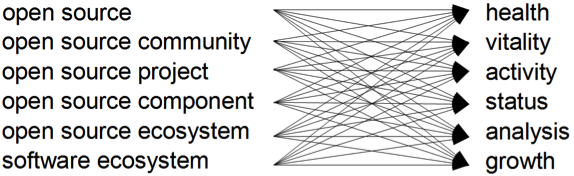
\includegraphics[scale=0.8]{figures/keyword_combinations.png}
\caption{Systematic Literature Review: Keyword combinations}
\label{fig:fig:keywords}
\end{center}
\end{figure}

The review excluded papers that exclusively focus on open source without ecosystem or health related perspectives. Papers solely describing the SECO domain, research agendas and similar work were also excluded, as these lack relevance for answering the research questions. Furthermore, a limitation to the first five pages of result pagination is applied. Due to the use of popular search terms, such as 'health' or 'open source', publication search engines can, at times, produce more than 25'000 results. Due to such manually not procelssible numbers, this exclusion criterion is designed with the assumption that the utilized ranking algorithms weigh papers, including a combination of multiple relevant search terms, greater than those only matching one keyword. Based on additional filtering features, search results on Microsoft Academic are limited to the domains of Computer Science and Economic \& Business. Results on Google scholar exclude results for patents. Further restrictions apply to language. The search was performed exclusively in English, articles in other languages than English, German or French were discarded.

The extraction process was performed as follows (see Figure \ref{fig:systematic_selection}). First, the titles of all scientific research (within the first five pagination results of Microsoft Academic and Google Scholar) were read. Titles matching the inclusion criteria, or those in question to potentially match the criteria were selected for closer review. Given the popularity of the individual keywords, only a small percentage of the discovered research was deemed relevant, as a vast number of research papers belonged to the domain of medical informatics or did not match the predefined criteria. Consequently, each abstract of the remaining selection of 121 titles was read. Having gained a deeper understanding of the research content of each paper, another 69 candidates have been discarded. The remaining 52 papers were fully read and further 22 discarded based on a lack of focus on OSC understanding, OSC vitality relevance or a sole focus on software ecosystems, without relevance to open source.
\begin{figure}[htp]
\begin{center}
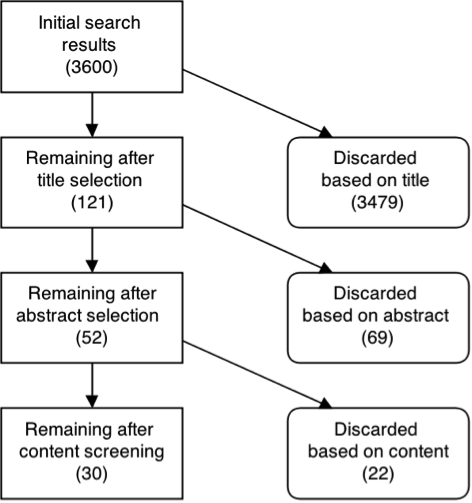
\includegraphics[scale=0.8]{figures/Systematic_literature_review.png}
\caption{Systematic Literature Review: Paper Selection Process}
\label{fig:systematic_selection}
\end{center}
\end{figure}
\section{Community Health and Vitality Indicators}
\label{OSC_vitality_section}
The following section introduces an exhaustive collection of theoretical and empirical OSC vitality indicators, originating from the performed systematic literature review and expert interviews, conducted at IBM. Table \ref{tab:vitality_indicators} depicts the indicator names, descriptions and their particular origin(s). The indicators can be seen as a high level conceptualization of a number of viewpoints or aspects of OS communities. It is important to highlight that all quantifiable attributes should be considered as relative values, dependent on respective OSC realities. For instance, online popularity or the total number of downloads can greatly vary between different types of communities. Despite low absolute indicators, a niche open source project with a small core team or a low number of total downloads can still be successful and healthy. This view is supported by recent OSC related publications that argue that the relative weight of vitality variables can vary between OS projects and that each variable should therefore be adjusted to the characteristic of its community \cite{Wahyudin2007}. Next to considerations for absolute or relative variables, another controversial OSC vitality indicator is the type of OSC license(s) a project is using to publish its source code. The controversy stems from the fact that it is unlikely that a software project manager would consider the utilization of licenses that are not suitable for commercial software applications, yet all types of OSC licenses can have different implications for community motivation. Due to their importance for OSC vitality, this section introduces OSC licenses as a valid vitality indicator; however the following OSC health analysis method is based on the assumption that software product managers will only utilize OSCs that are published under commercially acceptable terms, such as the MIT license. Finally, although covered by some of the reviewed literature approaches, no consideration is given to indicators, such as software category, the programming language or current trends in software development. Despite discovered correlations with community vitality \cite{Stewart2006}, each case had to be adjusted to the local realities of the respective OSCs, contemporary trends and other non-generic factors. The authors find such adjustments to be difficult to reproduce and hence exclude them from the list of suitable vitality indicators.


\begin{table*}
\label{tab:vitality_indicators}
    \begin{tabular}{|p{0.5cm}|p{2.5cm}|p{10cm}|p{3.5cm}|}
    \hline
    \textbf{ID}  & \textbf{Vitality Indicator}                                           & \textbf{Description}                                                      & \textbf{Origin}                           \\ \hline
    V1  & Activity Patterns                                            & Cyclic and seasonally dependent activities, cyclic and seasonally independent activities or acyclic activities.& Literature: \cite{Yu2009} \\ \hline

	V2  &Avg. duration before a bug fix& Research with software companies integrating OSCs showed that the response rate for bug fixes can be seen as an indicator for community activity. & Literature: \cite{Maki-Asiala2006}, Interviewees: 2 \& 4         \\ \hline    
    
    
   V3  &                   Community age                              & The longer a community exists, the less likely it is to be abandoned. Communities older than 5 years are considered mature and often exhibit similar software development processes as those practiced in commercial software firms                                                                                                            & Literature:\cite{Samoladas2010}, Interviewee: 5                \\ \hline
    V4  &                   (Core) developer reputation                &    Technical and leadership reputation of (core) developers of OSC projects                                                                                           & Literature:\cite{Immonen2007},  Interviewee: 2            \\ \hline
    V5  &                   Corporate Patronage                        & Research results suggest that sponsored OSC projects are more likely to become popular than non-sponsored ones                                                                    & Literatures:\cite{West2008} \& \cite{Stewart2005} \\ \hline
    V6  &                   Developer Interest and motivation          &                   Developer interest can be defined by:                   Altruistic reasons to contribute to a project,              an opportunity to improve skills in a technical domain or by financial gains from new or improved skills in a high demand domain. & Literature: \cite{Subramaniam2009} \& \cite{Wu2007}   \\ \hline
    V7  &                   Frequency of bug reports                   &                   Statistical evidence suggests that frequent bug reporting indicates an active community                                                                                                                                                                             & Literature: \cite{Raja2006}                      \\ \hline
   V8  &                   License restrictiveness                    & Restrictive licenses, such as GPL negatively correlate with activity levels of OSS projects                                                                                                                                                                                           & Literature: \cite{Stewart2005} \&\cite{Subramaniam2009},  Interviewees: 1, 2, 3, 4 \& 5              \\ \hline
   V9  & Maturity of Software development processes & Representative indicators are the utilization of publicly accessible version control, structured patch contribution processes, as well as similar software development practices. & Literature:\cite{Michlmayr2005} \& \cite{Maki-Asiala2006}, Interviewees: 2 \& 5               \\ \hline
    V10 &                   Number of committers                       &                   Absolute and relative number of code committers. Samoladas et al. estimate an increase in probability for project survival of 15.8 \% for every new committer \cite{Samoladas2010}                                                                                                                                                                                                                     & Literature: \cite{Samoladas2010} \& \cite{Crowston2003}, Interviewees: 1, 2 and 3                 \\ \hline
    V11 &                   Number of OSC downloads                    &                   Total and relative number of downloads and version management clones                   (e.g. via Git)                                                                                                                                                 & Literature:\cite{Raja2006} \& \cite{Maki-Asiala2006}          \\ \hline
   V12 &                   Online popularity                          & Expressed by:                   Trending Topics on search engines,              frequency of cross references in technical blogs or by other software projects or reputation within expert communities                                                                                & Literature: \cite{Weiss2005} \& \cite{Immonen2007}, Interviewees: 2 and 3              \\ \hline
    V13 &                   OSS code quality                           &                   Code inspections allow to approach uncertainties regarding OSC code quality and indicate skill level of OSC submitters.                                                                                                                                             & Literature: \cite{Maki-Asiala2006}, \cite{Parizi2010} \& \cite{Samoladas2008} \\
    ~   & ~                                                            &                   Interview results highlighted that code screening /review is a common measure for OSC evaluation                                                                                                                                                                    &                   Interviewees: 2 and 4                                          \\ \hline
    V14 &                   Project activity                           & Mailing list activity, forum activity, avg. time to respond to feedback, IRC or Git discussions. & Literagture: \cite{Subramaniam2009}, Interviewees: 1, 2, 3, 4 and 5                           \\ \hline
    V15 &                   Quality of OSC documentation               & Quality of functional OSC description and API documentation, as well as usability of code examples   & Interviewees: 2 and 4    \\ \hline
    V16 &                   Release frequency                          & Frequency of minor and major updates, including added functionality    & Interviewees: 1, 3 and 5   \\ \hline
    V17 &                   Size of core development team              & The Core team is vital for community health and drives and coordinates community activities                                                               & Literature: \cite{Torres2011} , Interviewee: 3   \\ \hline
    V18 &                   User interest in the project               & On short term, user interest has been found to positively influence developer interest and project activity                                                                & Literature: \cite{Subramaniam2009} \\ \hline
    \end{tabular}
    \caption{Open Source Community Vitality Indicators}
\end{table*}


\section{The OSC Health Analysis Method}
\label{OSC_method_section}
Built on the developed understanding of OSC vitality, this section introduces a systematic approach for software product managers that enables them to evaluate the vitality of candidate open source communities. Hereby, the foundation for the following method is based on five expert interviews, the introduced systematic literature review, a study of OSC related practices at the case company, as well as a distilled list of OSC vitality indicators.
\subsection{Method Fragment Pool}
\begin{figure*}
\begin{center}
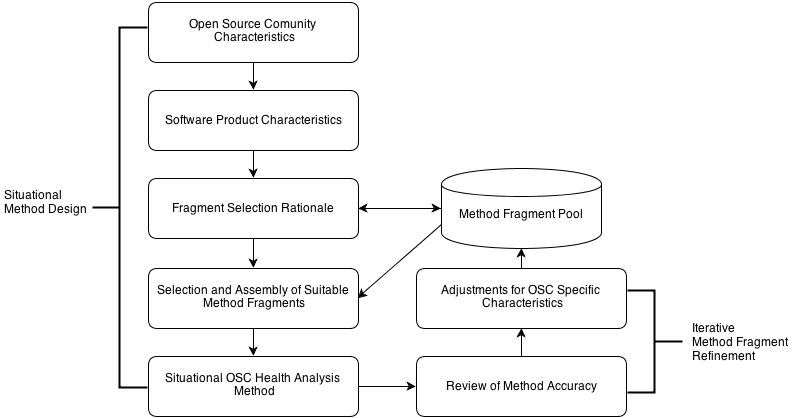
\includegraphics[scale=0.55]{figures/Situational_Method_Design.png}
\caption{Design Process: Situational OSC Health Analysis Method}
\label{fig:OSC_model}
\end{center}
\end{figure*} 
Derived from the domain of method engineering, this section introduces the concept of situational method design, as well as that of a method fragment pool, containing base elements for method assembly. While the general principles of situational method engineering \cite{VanDeWeerd2008} fully apply, this section focuses on a customized adoption towards the specific needs of Software Product Managers and their responsibilities in regard to OSC dependency management. Built upon the work of Harmsen, Brinkkemper and Oei \cite{Harmsen1994}, Figure \ref{fig:OSC_model} depicts a process flow aimed at creating a situational method for OSC vitality assessment. Furthermore, the diagram includes an iterative cycle, focused on the customization of method fragments towards a community's unique characteristics. The building blocks of a situational method are so called method fragments, which are stored within the method fragment pool. Each element within the pool focuses on assessing one specific OSC vitality aspect and can be either used by itself, or in combination with other fragments. Each fragment is linked to situational factors that make it best suited for assessing either a given community type or determining its applicability for a given Software Product. Fragment selection begins with an assessment of OSC characteristics, necessary for narrowing down the total number of candidate method fragments for the given case. Combined with the requirements and the resources of the respective Software Product, both form the selection rational for choosing suitable method fragments within the existing fragment pool. Following the selection process, the chosen fragments are being assembled into a situational method. Although a particular order is not a requirement, a logical structure or segmentation into fragment groups can contribute to the method’s usability. Depending on the relative significance of community aspects, fragment importance can vary. Thus, looking at the overall quality of the software product, individual fragments can receive a greater weighted influence over less significant ones. After method assembly, the individual fragments and the entire method can undergo an iterative process, aimed at improving the accuracy of the assessed OSC vitality. Hereby, historic or present community data can be used to review fragment and method accuracy. If a given fragment is found to generate inaccurate or contradictory vitality data it can be adjusted, its result weighed less or it can be fully removed from the situational method. All community specific adjustments can then be updated and re-­inserted into the fragment pool. Should another software product, with varying project characteristics, require assessing this particular OSC, the new and more accurate fragments can be implemented.

\subsection{Fragment Categorization and Selection Rationale}
The following sub-section introduces a number of criteria that can be used to select situation specific method fragments for a given OS community or software development project. The main reason for this approach is the intention to create a practical heuristic that can be quickly utilized for method assembly. The approach does not enforce the selection of specific fragments, based on the presented rationale, but merely suggests using it as an indicator for assessing fragment suitability. The three introduced criteria have been selected based on their simplicity for the use by software product managers and their universal applicability for varying types of OSCs. Herby, the first two indicators stem from scientific literature and focus on specific community characteristics. The third indicator is based on the authors’ estimate for required fragment resources and aims at a software product's development scope.

\begin{figure}[htp]
\begin{center}

\includegraphics[scale=0.15]{figures/situational_factor_community_size.PNG}
\caption{Fragment Selection Indicator - ­Community size}
\label{fig:ratio_community_soze}
\end{center}
\end{figure}
The most evident indicator for fragment selection is community size. Hereby the size can be measured by the number of OSC developers, the number of core developers or alternatively the total number of registered community members. While this indicator needs to be adjusted for each community's nature or characteristics, it can help to quickly exclude fragments that are only applicable to large or very small OSC types. Each method fragment is labelled with one or many community size indicators, suggesting the most suitable community sizes.

Community age is a direct indicator for the probability of its survival and was found to have a significant positive correlation with the maturity of it software development processes and its governance structure \cite{Samoladas2010}. This in return makes it a suitable indicator for selecting applicable method fragment, as it can indicate which fragments are best suited for mature or young OSCs. Alike to the previous indicator, each fragment can have one or multiple labels describing matching OSC criteria.
\begin{figure}[htp]
\begin{center}

\includegraphics[scale=0.15]{figures/situational_factor_community_maturity.PNG}
\caption{Fragment Selection Indicator - ­Community maturity}
\label{fig:ratio_community_maturity}
\end{center}
\end{figure} 
Looking directly at the perspective of software product managers, disposable time and financial resources can vary greatly with each managed software product. Thus, even if a method fragment for vitality assessment is promising, it yet may not be feasible to use. This can be the case if the given fragment exceeds available project resources or if the overall analysis would benefit from focusing the efforts on less resource intensive fragments. In contrast to the previous indicator, each fragment is labeled with only one cost indicator that expresses the authors' estimate of the necessary financial or time investment, in order to execute the according method fragment.
\begin{figure}[htp]
\begin{center}

\includegraphics[scale=0.15]{figures/situational_factor_resource_investment.PNG}
\caption{Fragment Selection Indicator - ­Fragment cost}
\label{fig:ratio_fragment_cost}
\end{center}
\end{figure}   
\subsection{Sample Fragment and Method Utilization}
\label{sub_section_method_utilization}
By combining the introduced selection rationale and a list of validated vitality indicators, this sub-section describes a representative OSC health method fragments that can be used by software product managers for OSC assessment. The complete method is comprised of ten method fragments, segmented into five fragment categories. Three categories are  designed to group fragments that operationalize and process similar data types. The remaining two categories aim at establishing a common method base for standardized data extraction and the optimization of monitoring resource with other OSC stakeholders.

The sample fragment, depicted in Figure \ref{fig:OSC_method_fragment}, aims at external OSC metrics and is most suitable for measuring outward facing OSC activities. This includes actions, such as extracting the number of OSC downloads over time, tracking online search popularity or monitoring release frequency. All activities produce individual results, as well as an aggregate index, representing the overall metrics performance. The fragment is suitable for a broad range of OSCs with varying degrees of maturity and size. However, due to the necessity to establish and track changes to the indices, the fragment is relatively expensive and has the second highest cost rating.
\begin{figure*}
\begin{center}
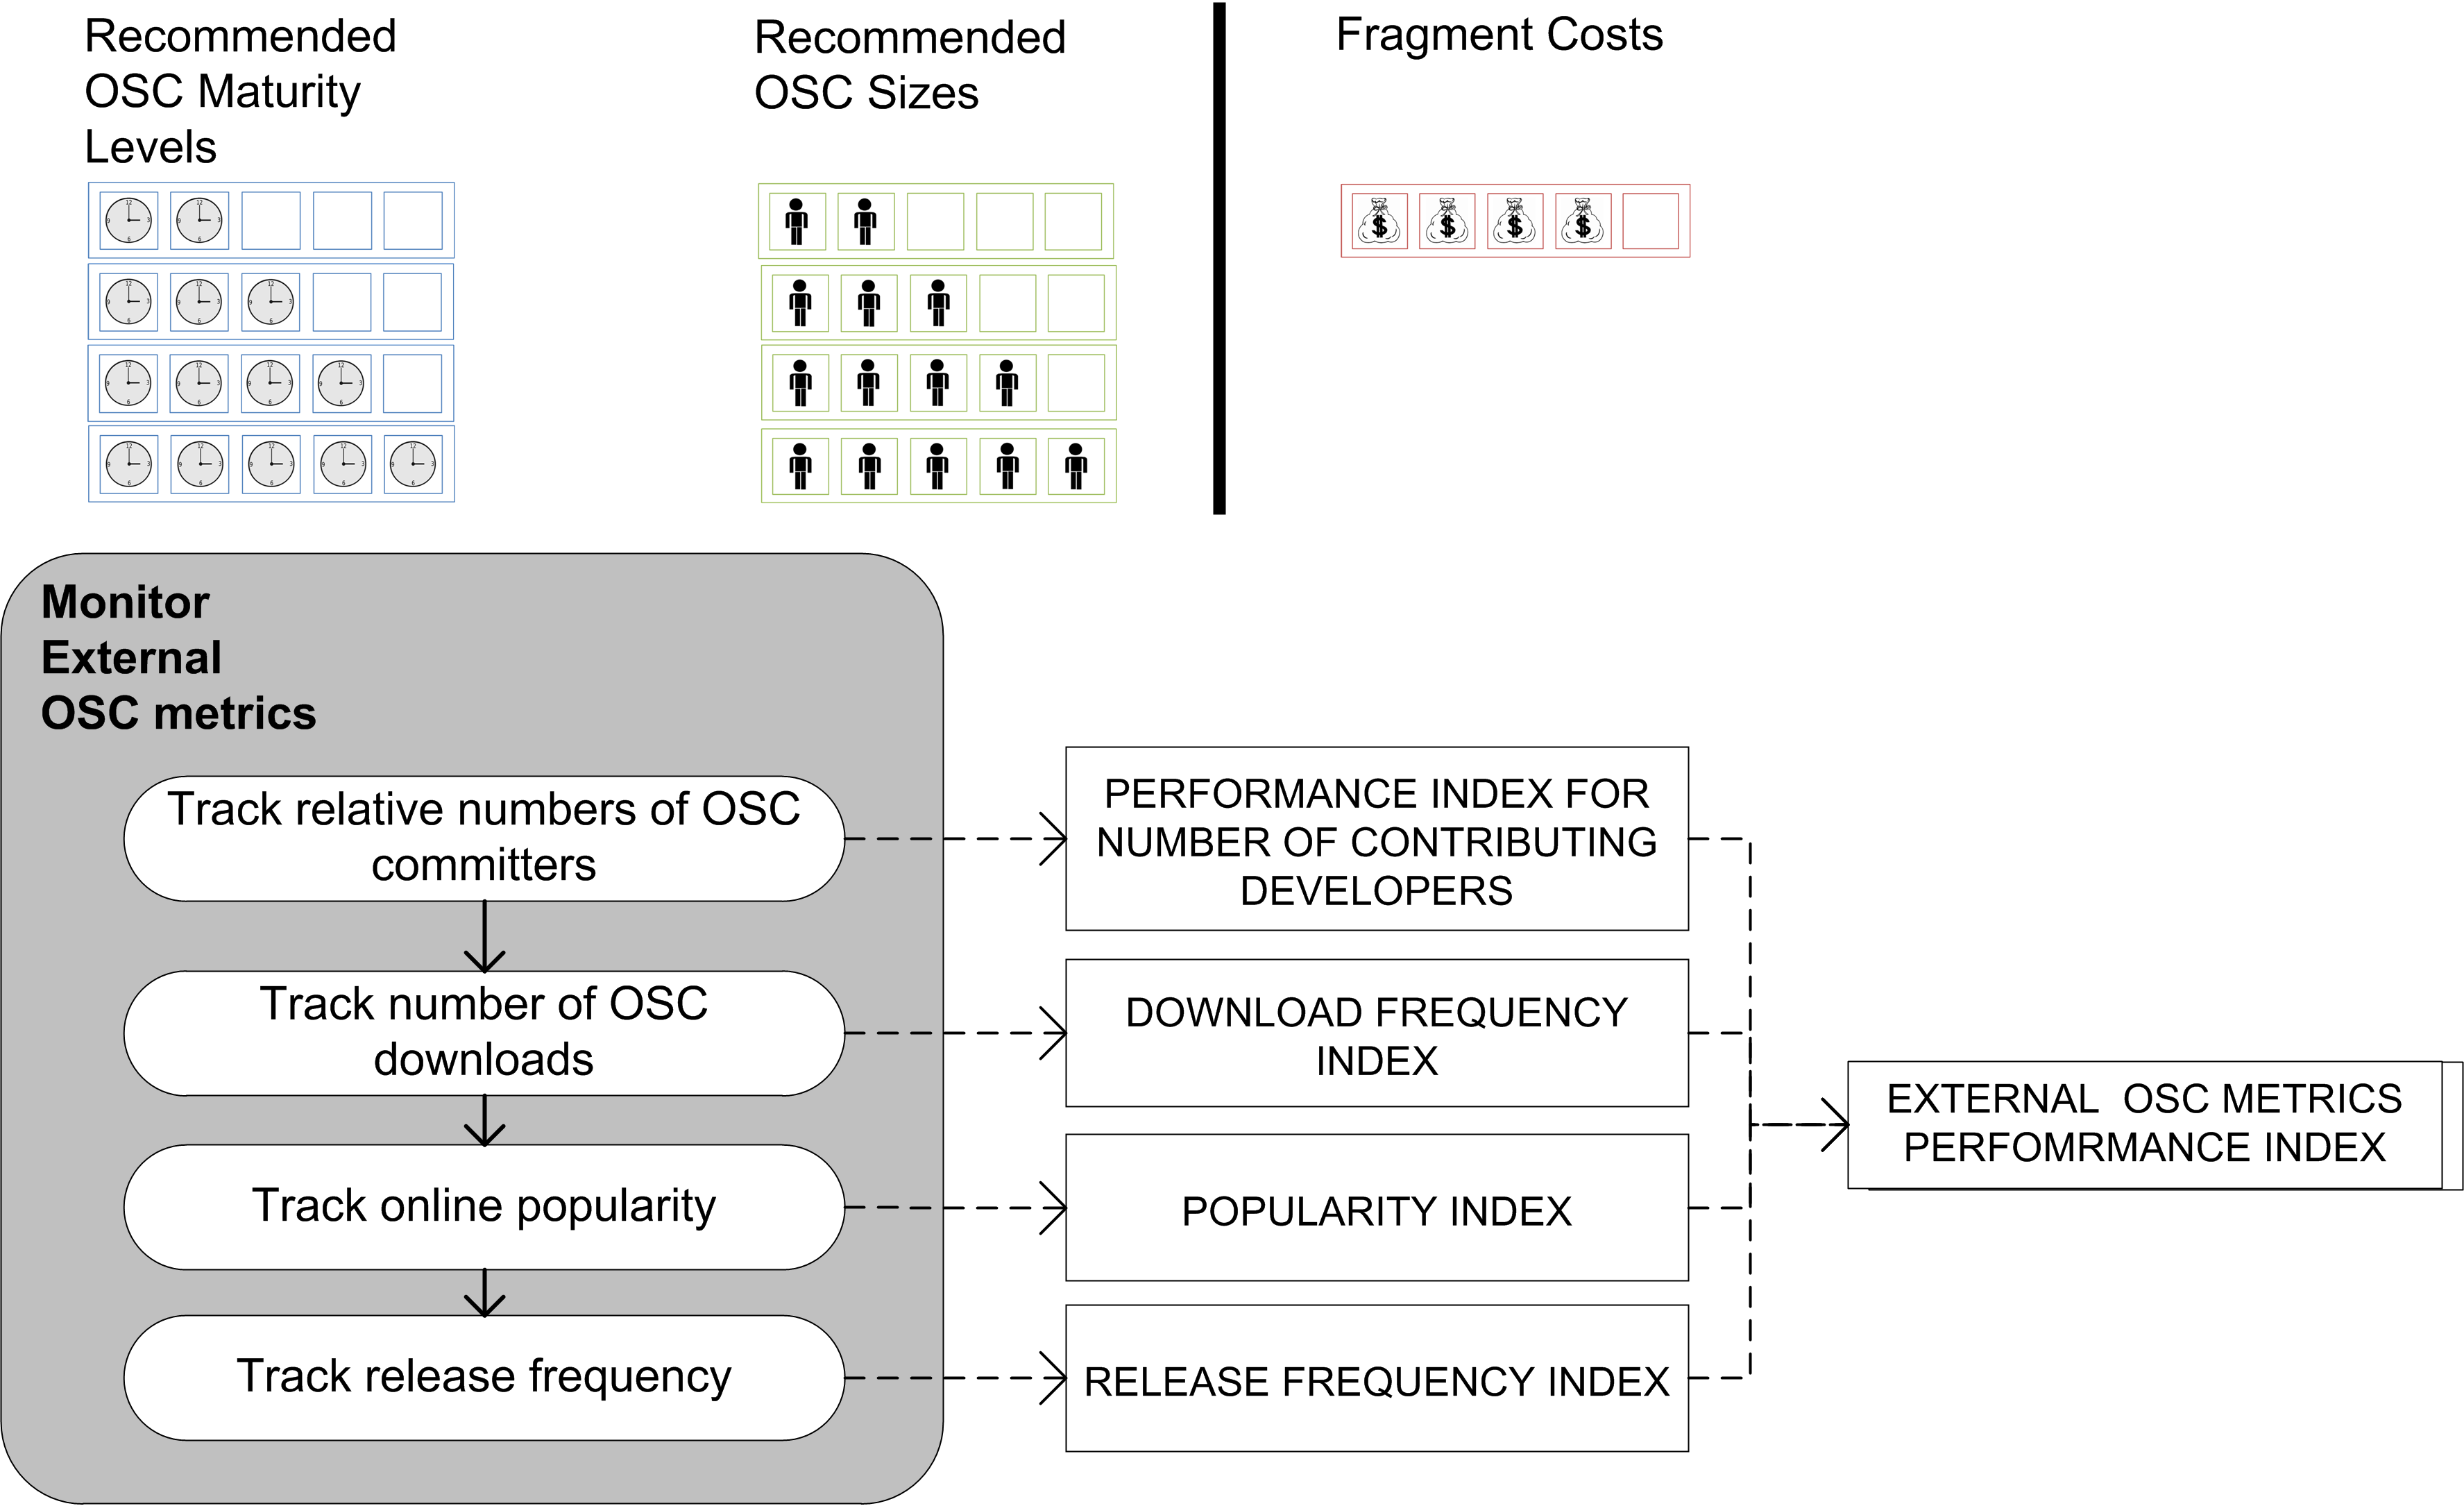
\includegraphics[scale=0.7]{figures/monitor_external_metrics.png}
\caption{OSC Health Method Fragment: Monitor external metrics}
\label{fig:OSC_method_fragment}
\end{center}
\end{figure*}   
In order to present a practical example of the method’s application, a representative OSC was selected for data analysis. The main reason for choosing a single OSC was to introduce a set of steps that can be taken in order to apply the introduced method fragments to a realistic assessment scenario. Furthermore, the aim was to present an analysis of a broadly known OSC and thus make the example as relatable as possible for project managers, familiarizing themselves with the new method. 

OSC selection was performed based on the popularity index of one of the most widespread public source code repositories, namely Github. The platform is built around the distributed revision control system Git that provides an additional source of data. Due to Git's fully distributed architecture, revision data can be directly extracted from every cloned copy of a repository. Among the highest rated community projects on Github, the jQuery JavaScript library was selected for analysis. Although ranked third in the index (8. May 2013), the first two projects Twitter Bootstrap and Node.js were excluded due to either their direct ties to a commercial entity or the scope of available data and community maturity.The fragment's analysis is based on community data available on Github, the jQery Git repository, Ohloh (a public directory of open source software owned by Black Duck Software, Inc.), as well as community pages, blog entries and similar documentation of the jQery project. The jQery Git repository was mined with the open source tool GitStats\footnote{http://gitstats.sourceforge.net}.

As suggested by the method fragment, all measured indices are aggregated into one external performance index. For this purpose, each metric has been first recorded with the according activity for each month between Aug. 07 and Apr. 13. Due to the different measuring units, the performance was adjusted to changes in percent, relative to a standardized base value. The index for the number of active contributors per month is operationalized by changes in percent, compared to an average of 8 contributors per month. This value is based on the actual project average for its entire lifespan and has been rounded to an integer value. Release frequency is recorded in relative frequency compared to a release frequency of 2 releases per year or 0.16 releases per month. As online popularity is already measured in percent values, relative to an established base value, the index has been included in the analysis as is. Although the most recent Github API does offer the opportunity to extract the overall number of downloads, this data attribute is not tracked over time and does not take downloads from other mirrors into account. Thus, this vitality indicator will not be included in this analysis.

By combining the external performance indicators with available data for commit frequency, an aggregate view can be generated that incorporates all long term community activity into a single performance index. Figure \ref{fig:OSC_performance_index} depicts a unified index that combines all measured external vitality indicators with OSC commit frequency. Hereby, the commit frequency is expressed in a relative percent value based on an average commit frequency of 60 commits per month.

It is noteworthy that when evaluating the graph, measurement consistency is most important while exact performance values lack significance. All index activity values are measured in relation to an established base value and could indicate stronger or weaker growth if the base is modified.
\begin{figure*}
\begin{center}
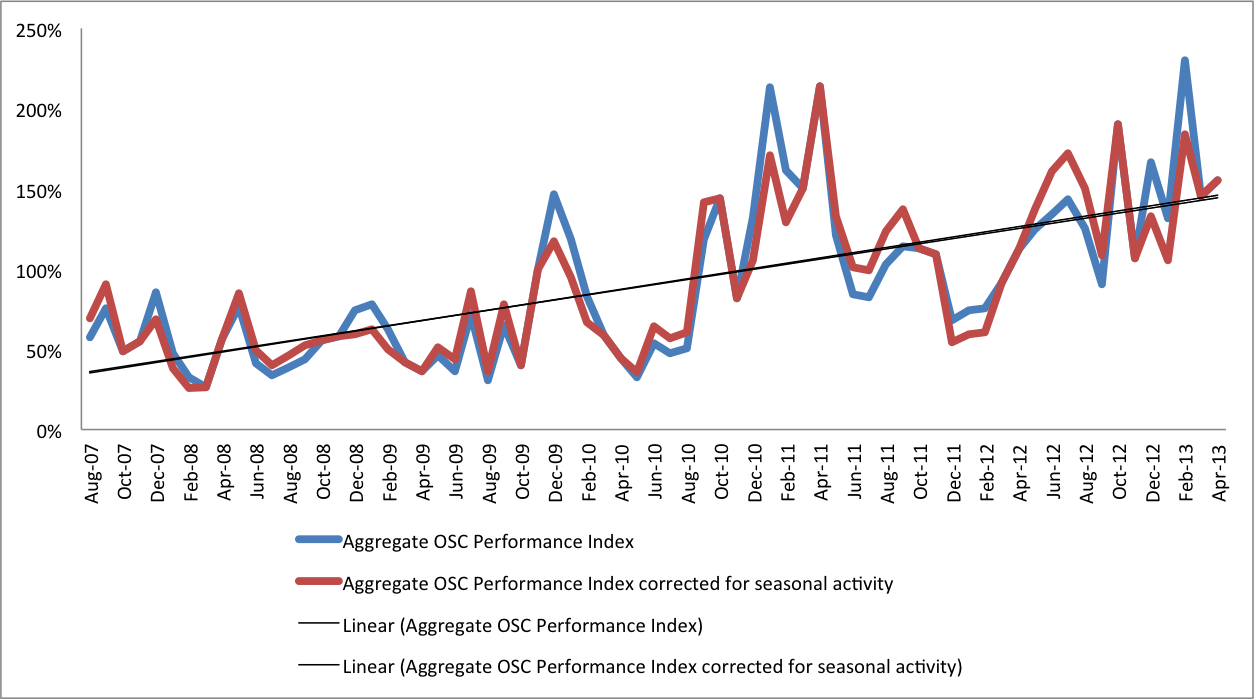
\includegraphics[scale=0.7]{figures/Aggregate_OSC_Performance_Index.png}
\caption{Aggregate OSC Performance Index: jQuery Core}
\label{fig:OSC_performance_index}
\end{center}
\end{figure*}   
\subsection{Method Assembly and Calibration}
Depending on fragment selection, the final situational method can contain any combination of index or scale based elements, as well as binary results. Additionally, two fragments with the purpose of either correcting activity indexes for cyclical trends or for optimizing OSC monitoring efforts can be included. 

The only fragment required for method assembly is the method base. Consequently, any number or combination of fragments can be utilized within the situational method. Based on the chosen selection rationale, software product managers can group fragments and are free to either aggregate method results or compare them on an individual basis. 

Specifically looking at index driven methods and the produced performance indices, they can be aggregated to create a unified OSC performance index. Next to the overall OSC health, individual vitality indicators can be monitored separately in order to identify trends within vitality areas. Furthermore, the approach supports index adjustment by correcting the individual weight of vitality indices according to their importance for a given OSC. Thus, a situational method cannot just be tuned by means of fragment selection but also by means of adjusting fragments to local OSC realities. 

Method artifacts generated by non-index fragments lack a distinct scale; however they can be used to register changes in vitality. By individually tracking variations in the likert ratings, each method fragment can be used as an indicator for changes in OSC health. The same applies to the specific case of monitoring software development practices. Despite the binary nature of the results, each can be compared to past practices of the OSC. Thus, added practices can be seen as an improvement to community health or code quality, while the abandonment of practices can be seen as a decline in community performance. 
\section{Method Suitability and Applicability}
\label{suitability_applicability__section}
The following section contains the evaluation results for the OSC Health Analysis Method.

In regard to the general value of applying a structured approach to OSC vitality analysis, virtually all interviewees stated that a more formal approach is preferred over the current individual ad-hoc analysis. Furthermore, seven interviewees stated that the introduced research domain and vitality analysis method raised their awareness for open source related risks and benefits. A majority of the interviewees mentioned that the presented method exceeds the current practices and rated the additional degree of information a valuable contribution to overall product quality.

Specifically looking at method usability, eight out of ten interviewees stated that they would be interested in applying the presented method in future open source related activities. Two interviewees stated that the method, while potentially more accurate than their current approach, would probably consume too much of their time and that they would prefer to rely on a more standardized tool or rating platform.

Specifically asked about the value and suitability of the presented vitality indicators, all interviewees agreed with the presented list and no objections or remarks were made. Furthermore, all interviewers stated their approval for the scientifically evaluated indicators. Particularly those interviewees already practicing OSC analysis, showed interest in the origin and potential applicability of indicators stemming from scientific research.

After having completed the task of assembling three situational methods for sample OSCs, the interviewees were asked to describe their experiences with the process. Hereby, the introduced scenarios covered the perspectives of a small IT service provider, a small or medium enterprise (SME), as well as a large product software developer.

For all three cases, fragment selection has been found to be clear and transparent. Specifically the three categories for the selection rationale were perceived positively by all interviewees. Hereby, eight interviewees mentioned a particular preference for the fragment cost indicator, followed by the recommended community sizes. Community maturity was generally understood, however it required some additional clarification during half of the interviews.

In contrast to fragment selection, fragment assembly was completed by all interviewees in a considerably speedier manner. Particularly those cases requiring a limited selection of method fragments were assembled within less than two minutes.

All interviewees acknowledged the benefits of adjusting fragments to the situational requirements of each monitored OSCs. Hereby, a number of concerns in regard to the accuracy of fragment measurements were raised. Index driven fragments were found to be most difficult to compare by six interviewees. All six mentioned that custom adjustments by one product manager might not be comparable to the results of another one, reviewing the same OSC. Concerns about calibration of index driven fragments were mentioned by four interviewees.

Asked if the interviewees would see themselves able to execute the assembled OSC Health Analysis methods, all confirmed their general capability to do so, however raised a number of concerns regarding a lack of practical experience in applying the method,  data availability, the willingness of OSC developers to participate in interviews or if the method is best applied on an individual or organizational level.
\section{Discussion and Conclusion}
\label{discussion_conclusion_section}
Analyzing open source vitality, this research introduced an Open Source Community (OSC) Health Analysis Method, specifically aimed at the needs of software product managers, handling open source components within their managed products. The introduced approach allows product managers to create custom vitality analysis methods that are adjusted to community characteristics and take available time and resources into consideration.

Eighteen validated vitality indicators and three selection indicators lay the foundation for a pool of method fragments that serves as the base for situational method design for OSC vitality analysis. The developed method has been validated by means of semi structured interviews, as well as exercises in method assembly by open source experts at the case company. The validation results confirm the method's general applicability for structured vitality analysis, as well as the utilized vitality indicators.

When reviewing the results, three limitations are particularly noteworthy and need to be kept in mind when reviewing the research results.

The individual vitality indicators have been thoroughly validated; however their implementation within the OSC Health Analysis Method is based on the authors' understanding of open source vitality and the needs of software product managers. Only further research and additional case studies or experiments can proof the suitability of the chosen method engineering approach.

Open source communities are often part of entire networks of communities that integrate components or libraries into larger software constructs. The OSC Health Analysis Method exclusively looks at one OSC at a time and does not review the influence of components stemming from other open source projects. Although it would be possible to apply the method to all OS based dependencies, such an approach is likely to be very resource intensive and could greatly complicate vitality analysis.

The introduced exemplary applicability of the OSC Health Analysis Method is not based on an actual case of OSC integration but was solely included as a reference to demonstrate one possible way of performing vitality analysis on a popular and widely known OSC. The way the method will be applied and reviewed by SPMs can be heavily influenced by the included examples.

%% The Appendices part is started with the command \appendix;
%% appendix sections are then done as normal sections
%% \appendix

%% \section{}
%% \label{}

%% References
%%
%% Following citation commands can be used in the body text:
%% Usage of \cite is as follows:
%%   \cite{key}          ==>>  [#]
%%   \cite[chap. 2]{key} ==>>  [#, chap. 2]
%%   \citet{key}         ==>>  Author [#]

%% References with bibTeX database:

\bibliographystyle{model1-num-names}
\bibliography{sources.bib}


\end{document}

%%
%% End of file `elsarticle-template-1-num.tex'.
